%%%%%%%%%%%%%%%%%%%%%%%%%%%%%%%%%%%%%%%%%%%%%%%%%%%%%%%%%%%%%%%%%%%%%%%%%%%%%%%
% Seismica submission manuscript -- shortened main paper, version 28
% Supporting detail and diagnostic figures are in supplement29.tex.
%%%%%%%%%%%%%%%%%%%%%%%%%%%%%%%%%%%%%%%%%%%%%%%%%%%%%%%%%%%%%%%%%%%%%%%%%%%%%%%

\documentclass[]{seismica}
\usepackage{tabularx}
\usepackage{placeins}

% Compile from the repository latex/ directory.
\graphicspath{
  {../data/outputs/170_generate_publication_figures/}
  {../data/outputs/145_analyze_regional_detectability/}
  {../data/outputs/140_search_for_direct_seismic_waves/}
  {../data/outputs/130_analyze_seismic_polarization/}
  {../data/outputs/120_estimate_acoustic_energetics/}
  {../data/outputs/110_measure_named_events/}
  {../data/outputs/100_measure_event_amplitudes_and_acoustic_seismic_coupling/figures/}
  {../data/outputs/100_measure_event_amplitudes_and_acoustic_seismic_coupling/}
  {../data/outputs/090_analyze_finite_distance_propagation/}
  {../data/outputs/080_analyze_planar_array_propagation/}
  {../data/outputs/040_validate_event_catalogue_with_array_processing/figures/}
  {figures/}
}

% These boxes keep the manuscript compilable while the two remaining main
% figures are regenerated. They should not appear in a submitted PDF.
\newcommand{\pendingfigure}[1]{%
  \fbox{\parbox[c][55mm][c]{0.92\textwidth}{\centering\textbf{Pending figure}\par#1}}}

\title{Close-Range Seismo-Acoustic Observations of the 2016 Falcon 9 AMOS-6 Failure at Cape Canaveral}
\shorttitle{Close-range observations of the 2016 Falcon 9 explosion}

% Confirm department-level present affiliations for Farrell and Mehta before
% submission.
\author[1]{Glenn Thompson\thanks{Corresponding author: \texttt{thompsong@usf.edu}; ORCID: 0000-0002-9173-0097}}
\author[2,3]{Robert G. Brown}
\author[1,4]{Alexandra Farrell}
\author[2,3]{John Kiriazes}
\author[1]{Stephen R. McNutt}
\author[1,5]{Christopher Mehta}
\affil[1]{School of Geosciences, University of South Florida, Tampa, Florida, USA}
\affil[2]{NASA Kennedy Space Center, Florida, USA}
\affil[3]{Present address: Florida Space Institute, University of Central Florida, Orlando, Florida, USA}
\affil[4]{Present address: University of Alaska Fairbanks, Fairbanks, Alaska, USA}
\affil[5]{Present address: Howard University, Washington, DC, USA}

\credit{Conceptualization}{Glenn Thompson, Stephen R. McNutt}
\credit{Methodology}{Glenn Thompson}
\credit{Software}{Glenn Thompson}
\credit{Validation}{Glenn Thompson}
\credit{Formal Analysis}{Glenn Thompson}
\credit{Investigation}{Glenn Thompson, Robert G. Brown, Alexandra Farrell, John Kiriazes, Stephen R. McNutt, Christopher Mehta}
\credit{Resources}{Robert G. Brown, John Kiriazes}
\credit{Data Curation}{Glenn Thompson}
\credit{Visualization}{Glenn Thompson}
\credit{Project Administration}{Glenn Thompson, Robert G. Brown, John Kiriazes}
\credit{Supervision}{Stephen R. McNutt}
\credit{Writing - Original draft}{Glenn Thompson}
\credit{Writing - Review \& Editing}{All authors}

\begin{document}

\makeseistitle{
  \begin{summary}{Abstract}
  On 1 September 2016, a Falcon~9 and its AMOS-6 payload were destroyed
  during propellant loading before a planned static-fire test at Space Launch
  Complex~40, Cape Canaveral. A broadband seismometer and three-element
  infrasound array 1.4~km away recorded the complete accident sequence. We
  reconstructed its chronology, searched approximately 37~h of preceding data
  for energetic precursors, and measured source direction, propagation,
  pressure, ground motion, and acoustic--seismic coupling. The catalogue
  contains 153 accepted multichannel pressure transients distributed among
  four phases over 26~min; it is a chronology, not a count of independent
  explosions. No attributable coherent impulsive precursor was detected. The
  principal explosion occurred 3.60~s after the initial upper-stage event and
  produced median positive and peak-to-peak pressures of 1.392 and 1.549~kPa.
  High-quality array solutions pointed toward the launch complex and gave a
  coherence-weighted apparent velocity of 352.0~m~s$^{-1}$, matching the
  meteorological prediction of 351.0~m~s$^{-1}$. Among 46 well-measured
  events, pressure and three-component peak ground velocity were nearly
  proportional ($b=0.962$, $R^2=0.953$). The observations demonstrate how a
  small close-range array can independently document a complex launch-site
  failure.
  \end{summary}
  %
  \begin{summary}{Non-technical summary}
  A seismic and low-frequency sound station approximately 1.4~km from the
  launch pad recorded the 2016 Falcon~9 accident at Cape Canaveral. The
  recordings independently show when energetic activity began, how the
  sequence developed, how large its strongest signals were, and whether the
  pressure waves came from the launch complex. No unusual coherent impulsive
  signal attributable to the accident was found during the preceding 37~h.
  The accident was not a single explosion: 153 accepted multichannel pressure
  transients occurred in four phases over approximately 26~min, although some
  closely spaced entries are different peaks within the same physical event
  complex. The strongest explosion followed the first upper-stage signal by
  3.60~s. Independent measurements of arrival direction and speed agree with
  propagation from the launch pad under the observed weather conditions. The
  study shows that a small continuously recording geophysical array can
  provide a calibrated, independently timed forensic record when access to a
  launch site is restricted and engineering telemetry is unavailable.
  \end{summary}
}

\section{Introduction}
\label{sec:introduction}

Rocket launches generate strong atmospheric and ground-motion signals, but
catastrophic launch failures are rarely recorded at close range by calibrated
seismic and infrasound instruments. Most seismo-acoustic studies of major
technological explosions have instead used regional observations, for which
atmospheric ducting and attenuation strongly influence arrival times and
amplitudes \citep{ottemoller_2008,green_2008,ceranna_2009,smink_2019,
pilger_beirut_2021,kim_pasyanos_2022}. Rocket-focused studies demonstrate
complementary capabilities: routine launches are detectable infrasonically at
large distances \citep{pilger_rocket_2021}, dense seismic deployments can
resolve launch-generated body and surface waves
\citep{schuster_rocketquake_2025}, and regional infrasound can locate and
estimate the effective yield of a large static-fire explosion
\citep{silber_scamfer_newglenn_2026}.

On 1 September 2016, a Falcon~9 was destroyed during propellant loading in the
countdown for a planned static-fire test at Space Launch Complex~40 (SLC-40),
Cape Canaveral Air Force Station (now Cape Canaveral Space Force Station),
Florida. The AMOS-6 payload was lost and the launch complex was extensively
damaged. The only publicly available original recording is the 5-min-40-s raw
USLaunchReport video and camera audio \citep{uslaunchreport_amos6_video_2016};
an edited analysis by \citet{manley_spacex_explosion_2016} was used only for
context.

The University of South Florida (USF) BCHH station, approximately 1.4~km from
SLC-40 on adjacent Kennedy Space Center property, fortuitously recorded the
complete sequence. The original forensic analysis was reported confidentially
to SpaceX in 2016 before detailed engineering findings were public. The
geophysical chronology was therefore developed independently of the later
root-cause determination.

The central advantage of this dataset is the combination of continuous
recording, physical calibration, array geometry, and proximity. It permits
subsecond timing and local pressure--ground comparisons that are usually
unavailable at regional distances, while public imagery provides an
independently inspectable record of selected physical stages. It also exposes
important limitations: one compact array can constrain direction and apparent
speed but not source range, and it cannot assign every later transient to a
specific vehicle or pad component.

Here we use the BCHH observations to test for a detectable energetic
precursor, reconstruct the accident chronology, measure the strongest events,
evaluate source direction and acoustic propagation, and characterize local
pressure--ground coupling. A separate regional search tests whether the
principal explosion can be associated with publicly archived records at much
greater distances. The broader objective is to establish which forensic
inferences a modest open geophysical deployment can support independently and
which still require engineering telemetry, denser spatial sampling, or
detailed atmospheric modelling at this unusual observational scale. We use
\emph{close range}, rather than the strict
acoustic term \emph{near field}: a 1.4-km wavelength at 350~m~s$^{-1}$
corresponds to approximately 0.25~Hz, below the principal analysis band.
Supporting methods, diagnostics, and sensitivity results are provided in the
Supplementary Material.

\section{Data and instrumentation}
\label{sec:data}

\subsection{BCHH array and geometry}

BCHH comprised a three-component Nanometrics Trillium Compact Posthole
seismometer near the centre of a three-element infraBSU pressure array with an
aperture of approximately 30~m (Figure~\ref{fig:site_array}). All six channels
were recorded continuously at 250~Hz by a GPS-synchronized Nanometrics
Centaur. The seismometer was buried approximately 0.5~m; the pressure sensors
were mounted 20--30~cm above ground.

On 6 October 2016, as Hurricane Matthew approached KSC, co-author Robert G.
Brown removed the three pressure sensors, electronics enclosures, and solar
panels; the buried seismometer remained in place. Because the pressure sensors
had not been formally surveyed before their precautionary removal, their
geometry was subsequently reconstructed from the surveyed cable-end locations.
Relative position errors of approximately 1--2~m are therefore plausible.
Source distances ranged from 1408.3 to 1440.0~m
(Table~\ref{tab:instrument_calibration}). DD2 was used as the reference
pressure channel.

\begin{figure*}[!tbp]
  \centering
  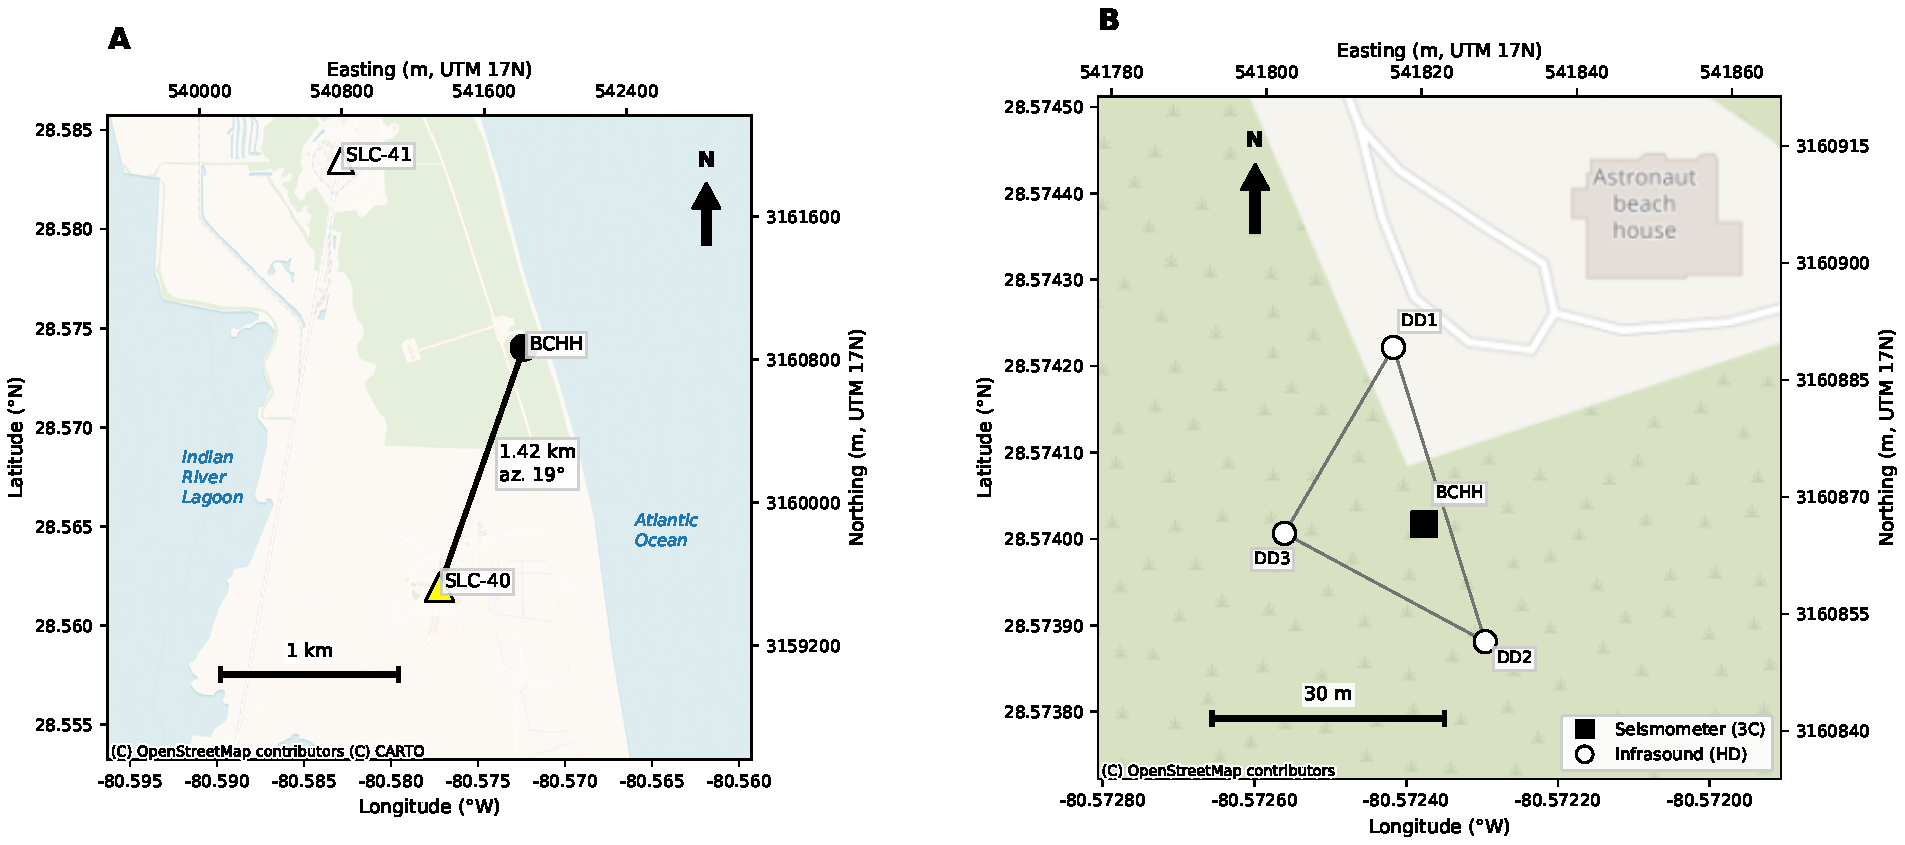
\includegraphics[width=0.96\textwidth]{fig01_slc40_bchh_location.pdf}
  \caption{Location and geometry of the BCHH seismo-acoustic array.
  (a) SLC-40 and BCHH in the southern Kennedy Space Center--Cape Canaveral
  launch area. (b) Three-component seismometer and three-element infrasound
  array. Pressure-sensor positions were reconstructed from surveyed cable ends,
  giving metre-scale relative-position uncertainty.}
  \label{fig:site_array}
\end{figure*}
\FloatBarrier

\subsection{Calibration, weather, video, and regional data}

The seismic response was removed using the manufacturer calibration for the
Trillium Compact Posthole--Centaur chain. Pressure channels were calibrated
individually using comparative vertical-displacement and impulsive tests of 25
USF infraBSU sensors. The adopted factors are listed in
Table~\ref{tab:instrument_calibration}; approximately $\pm20\%$ is treated as
the estimated field-calibration uncertainty of absolute pressure-dependent
quantities. Manual arrival uncertainty was approximately 0.01~s for the
clearest impulses and greater for weak, emergent, or overlapping signals. 

The USLaunchReport footage provided the public visual and camera-audio record.
Four proprietary videos obtained from SpaceX assisted and confirmed visual
interpretation but contained no usable audio and supplied no quantitative
result reported here. Data were sought from an infrasound array at CCAFS
operated by the Air Force Technical Applications Center (AFTAC) were sought
but were ultimately reported to have been lost. Regional pressure records to 1800~km
and vertical seismic records to 600~km were obtained through EarthScope FDSN
services; IU.DWPF, 97.7~km from SLC-40, was the nearest permanent station
examined \citep{asl_gsn_iu_1988}. 

Kennedy Space Center weather-tower observations supplied temperature,
relative humidity, and wind profiles at seven 5-min epochs from 13:05 to
13:35~UTC. Across the available observations, mean temperature was
26.4$\pm0.3\,^{\circ}$C and mean relative humidity was
83.9$\pm3.7\%$. The overall vector-mean wind was 5.4~m~s$^{-1}$ from
144$^\circ$. Vector-mean speeds at the seven epochs ranged from 5.25 to
5.46~m~s$^{-1}$, with a temporal standard deviation of only
0.09~m~s$^{-1}$; directions ranged from 142$^\circ$ to 149$^\circ$.
Atmospheric profiles and temporal variability are shown in Supplementary
Figures~S1 and~S2.

\begin{table*}[!tbp]
\centering
% Verify the notably lower DD2 counts-per-Pa factor against the archived
% calibration record before submission. If valid, explain the sensor/gain
% difference in the Data section or repository calibration note.
\caption{BCHH instrument channels, source--receiver geometry, sampling rate,
and calibration factors. Distance and azimuth are measured from SLC-40;
azimuth is clockwise from north. InfraBSU sensitivities are empirical field
calibrations.}
\label{tab:instrument_calibration}
\begin{tabular}{lrrrr}
\hline
Instrument/channel & Distance (m) & Azimuth ($^\circ$) & Sampling rate & Sensitivity \\
\hline
Trillium Compact DHZ/DHN/DHE & 1419.9 & 19.44 & 250~Hz
  & $3.0172\times10^8$ counts $(\mathrm{m\,s^{-1}})^{-1}$ \\
infraBSU DD1 & 1440.0 & 18.99 & 250~Hz & 8.10 counts~Pa$^{-1}$ \\
infraBSU DD2 & 1408.3 & 19.94 & 250~Hz & 0.690 counts~Pa$^{-1}$ \\
infraBSU DD3 & 1412.9 & 18.76 & 250~Hz & 10.0 counts~Pa$^{-1}$ \\
\hline
\end{tabular}
\end{table*}
\FloatBarrier

\section{Methods}
\label{sec:methods}

The analysis was implemented in Python as a reproducible sequence of Jupyter
notebooks \citep{kluyver2016jupyter}. Shared configuration and intermediate
products supplied common geometry, event times, propagation corrections, and
analysis parameters. Additional implementation and sensitivity details are in
Supplementary Sections~S1--S7.

\subsection{Waveform preparation and meteorological reduction}

Response removal used a 0.02, 0.05, 80, and 100~Hz four-corner prefilter and a
60-dB water level. A centred 1.0-s moving median was then removed independently
from each pressure channel to suppress slow baseline variation without an
additional physical-amplitude high-pass filter. Seismic traces remained in
ground velocity and pressure traces in Pa.

Using the mean temperature and humidity described in Section~2.2, the
still-air sound speed was 348.3~m~s$^{-1}$. Wind vectors were projected onto
the SLC-40--BCHH propagation direction. The available lower-atmosphere profile,
summarized over the nominal 0--65-m source-height interval, gave a vector-mean
wind of 4.6~m~s$^{-1}$ from 145$^\circ$ and a path-parallel tailwind component
of 2.6~m~s$^{-1}$. Because the lowest valid wind observations were near 40~m,
this lower-path estimate does not directly sample the entire surface layer.
Effective acoustic speed was calculated as
\begin{equation}
 c_{\mathrm{eff}}=c_0+\mathbf{u}\boldsymbol{\cdot}\hat{\mathbf{r}}.
 \label{eq:effective_speed}
\end{equation}
The calculated effective acoustic speed was 351.0~m~s$^{-1}$, which was used
for source-to-BCHH travel-time reduction.
Three time coordinates were kept distinct: observed
receiver UTC, DD2-referenced reduced arrival time, and source time. For sensor
$i$,
\begin{equation}
 t_{i,\mathrm{red}}=t_i-\frac{r_i-r_{\mathrm{DD2}}}{c_{\mathrm{eff}}}.
 \label{eq:reduced_time}
\end{equation}
Thus, catalogue times used for event association represent arrivals reduced
to DD2. Source times were calculated separately by subtracting the complete
source-to-DD2 acoustic travel time.

\subsection{Catalogue construction and quality control}

Manual pressure picks were mapped to the canonical DD1--DD3 geometry and
associated after differential travel-time reduction. A 0.040-s coincidence
window was selected as the smallest value on a stable association-count
plateau; a retained catalogue entry required picks on at least two channels.
Candidate waveforms were reviewed for signal-to-noise ratio (SNR), correlation,
and a coherent counterpart on the remaining channel. The catalogue records
accepted multichannel pressure transients, not independently verified physical
explosions.

Catalogue membership was separated from waveform quality. The
usable-waveform subset required robust peak SNR $\geq3$ and DD2--DD3
correlation $\geq0.5$; the core subset required SNR $\geq5$ and correlation
$\geq0.7$. Time-domain propagation quality was classified independently of
these waveform criteria. The high-quality planar class required maximum
coherence $\geq0.90$, back-azimuth standard deviation
$\leq0.5^\circ$, and apparent-speed standard deviation
$\leq3.0$~m~s$^{-1}$ across nine perturbations of the event scoring window.
Intermediate solutions used corresponding thresholds of 0.75,
1.0$^\circ$, and 8.0~m~s$^{-1}$.

Independent frequency-domain Bartlett beamforming was performed with LANL
InfraPy version~0.4.1.0 \citep{webster_infrapy_2025}, using all three pressure
channels. The primary validation used 0.5-s windows centred on the catalogue
times and a 2--20-Hz band. If $C$ is multichannel coherence for $N=3$
sensors, the array statistic was
\begin{equation}
 F=\frac{(N-1)C}{1-C}.
\end{equation}
An empirical threshold was defined as the 99.5th percentile of 153 pre-event
background windows, corresponding to $F=3.02$. A separate scan of 17,839
overlapping windows, positioned without reference to catalogue times, tested
catalogue recovery and searched for additional coherent activity.

\subsection{Propagation, amplitude, and coupling analyses}

A time-domain planar-wave grid search estimated back azimuth and apparent
velocity by maximizing multichannel waveform agreement. All catalogue entries
were processed, while physical interpretation emphasized quality-controlled
solutions. A fixed-source circular-wavefront calculation tested sensitivity to
the 1.4-km source range; because the three-element array provides only two
independent relative delays, it was not expected to resolve both source range
and propagation speed.

For each event, peak-to-peak pressure was measured from the differentially
aligned channels and three-component vector peak ground velocity (PGV) was
measured over a pressure-defined seismic window. A log--log model
\begin{equation}
 \log_{10}p_{\mathrm{p2p}}=a+b\log_{10}(\mathrm{PGV})
 \label{eq:power_law}
\end{equation}
was fitted to events satisfying independent pressure-SNR, seismic-SNR, and
window-capture criteria; uncertainty was estimated by event bootstrap.

Frequency-dependent coupling was described by the H1 pressure-to-vertical-
velocity estimator
\begin{equation}
 H_1(f)=\frac{S_{pv}(f)}{S_{pp}(f)},
 \label{eq:h1_transfer}
\end{equation}
with magnitude-squared coherence and permutation-derived empirical null
thresholds. Event and continuous Phase~I estimates overlap in time and were
treated as complementary rather than independent.

Named-event acoustic exposure was integrated over manually reviewed windows.
Assuming hemispherical radiation without atmospheric attenuation,
\begin{equation}
 E_{2\pi}=\frac{2\pi r^2}{\rho c}\int p^2(t)\,dt.
 \label{eq:acoustic_energy}
\end{equation}
Acoustic TNT equivalence is $E_{2\pi}/(4.184\times10^6~\mathrm{J\,kg^{-1}})$.
Any total-yield value additionally assumes an acoustic efficiency and is an
illustrative scenario, not a calibrated blast yield. Overlapping catalogue
windows were not summed as independent events.

\subsection{Video, regional, and polarization analyses}

The USLaunchReport recording lacks absolute UTC. Its first visible upper-stage
flash was mapped to the independently reduced BCHH chronology. Camera audio
was advanced by its 12.16-s path travel time, calculated from a 4.255-km range
and a camera-path effective speed of 349.8~m~s$^{-1}$. BCHH traces were reduced
using sensor-specific distances and 351~m~s$^{-1}$. Video supplied physical
labels for selected stages but was not used to construct the general catalogue.

Regional screening used broad physically plausible acoustic-celerity and
seismic-velocity windows. Candidate windows had to exceed matched pre- and
post-event controls and were then reviewed manually. Association required a
physically consistent multi-station branch; missing data or response failures
were not counted as non-detections.

Ground velocity was rotated into vertical, radial, and transverse components
using the 199.438$^\circ$ source back azimuth. A focused causal-filter search
examined 0.8--3, 3--8, 8--20, and 20--45~Hz between the upper-stage source time
and the larger principal explosion at +3.601~s. Amplitude-gated trailing
polarization windows prevented future samples from influencing an onset
estimate. Because only one station was available, no unique $P$, $S$, or
surface-wave phase was assigned.

\section{Results}
\label{sec:results}

\subsection{Atmosphere, catalogue, and temporal evolution}

Mean air temperature was 26.4$\pm0.3\,^{\circ}$C and mean relative humidity
83.9$\pm3.7\%$. The still-air speed was 348.3~m~s$^{-1}$ and the lower-profile
tailwind component was +2.6~m~s$^{-1}$, giving
$c_{\mathrm{eff}}=351.0$~m~s$^{-1}$. The 1419.9-m travel time was approximately
4.05~s, about 0.03~s shorter than the still-air estimate.

The final catalogue contains 153 accepted multichannel pressure transients:
48 in Phase~I, 4 in Phase~II, 96 in Phase~III, and 5 in Phase~IV
(Figure~\ref{fig:overview}). Of these, 138 met usable-waveform and 107 met core
criteria. The independently defined planar classes contained 51 high-quality,
45 intermediate, and 57 weak or broad solutions. Median robust peak SNR was
7.86, median DD2--DD3 correlation 0.876, and median corrected span among
associated picks 4.87~ms. These nested counts serve different analytical
purposes and none is a direct count of independent explosions.

No coherent multichannel impulsive precursor attributable to the accident was
identified during approximately 37~h before the first signal. This excludes
neither weak nor non-seismo-acoustic internal processes. No additional
explosion-related impulses were found during 10.5~h after Phase~IV. A
continuous signal lasting approximately 3.5~min followed Phase~I; its source is
not uniquely resolved.

\begin{figure*}[!tbp]
  \centering
  \includegraphics[width=0.98\textwidth]{fig03_bchh_30min_overview_zp_true.pdf}
  \caption{Thirty-minute BCHH overview. The upper traces are pressure and the
  lower traces are three-component ground velocity. Phase intervals and the
  prolonged seismic-dominant signal are marked; Phases I--IV contain 48, 4,
  96, and 5 catalogue transients.}
  \label{fig:overview}
\end{figure*}
\FloatBarrier

\subsection{Opening sequence and key events}

Four opening-sequence signals were assigned physical interpretations from the
mapped video chronology (Table~\ref{tab:principal_events}). The upper-stage
event occurred at 13:07:11.913~UTC. The principal explosion followed 3.601~s
later and produced the largest acoustic and seismic amplitudes: median positive,
negative, and peak-to-peak pressures were +1.392~kPa, $-157$~Pa, and
1.549~kPa, and vector PGV was
$3.57\times10^{-3}$~m~s$^{-1}$. The two payload-related signals were separated
by 0.568~s. Event~024 at 13:07:26.458~UTC had comparable amplitude but no unique
physical process could be assigned from the available video; it remains a
catalogue event rather than a fifth named stage.

Figure~\ref{fig:multimodal} shows that the first visible flash, reduced camera
audio, pressure, and ground motion are mutually consistent within the timing
limitations. Source times depend on the 351~m~s$^{-1}$ reduction, and the
video's mapped UTC remains conditional on the visual anchor.

\begin{figure*}[!tbp]
  \centering
  \includegraphics[width=0.98\textwidth]{fig04_multimodal_alignment_upper_stage.pdf}
  \caption{Video, camera audio, pressure, and ground-velocity alignment for
  the upper-stage event. Camera audio was advanced by its path travel time and
  BCHH traces by sensor-specific travel times. Pressure is baseline corrected;
  seismic traces are response corrected without an additional display filter.
  Traces are independently normalized. Video frames copyright 2016
  USLaunchReport.com/Michael Wagner; reproduced with permission
  \citep{uslaunchreport_amos6_video_2016}.}
  \label{fig:multimodal}
\end{figure*}

\begin{table*}[!tbp]
\caption{Physically interpreted opening-sequence signals. Pressure values are
medians of three sensor-specific measurements. Peak level is referenced to
20~$\mu$Pa. Event~024 and all catalogue-quality measurements are reported in
Supplementary Data Table~S1.}
\label{tab:principal_events}
\centering
\small
\begin{tabularx}{\textwidth}{Xcccccc}
\hline
Signal & \shortstack{Source time\\(UTC)} & $p_+$ (Pa) & $p_-$ (Pa) & $p_{\mathrm{p2p}}$ (Pa) & \shortstack{$L_{\mathrm{peak}}$\\(dB)} & \shortstack{Vector PGV\\(m s$^{-1}$)} \\
\hline
Upper-stage event & 13:07:11.913 & 38.8 & $-25.4$ & 77.1 & 125.8 & $7.85\times10^{-5}$ \\
Principal explosion & 13:07:15.514 & 1392 & $-157$ & 1549 & 156.9 & $3.57\times10^{-3}$ \\
Payload impact & 13:07:24.420 & 279.1 & $-115.3$ & 390.7 & 142.9 & $6.98\times10^{-4}$ \\
Post-impact explosion & 13:07:24.988 & 297.0 & $-113.4$ & 410.6 & 143.4 & $9.02\times10^{-4}$ \\
\hline
\end{tabularx}
\end{table*}
\FloatBarrier

\subsection{Waveforms, array propagation, and coupling}

The 51 events in the high-quality planar class show broadly repeatable
compression followed by a smaller rarefaction, whereas vertical ground
velocity has a longer oscillatory coda (Figure~\ref{fig:waveform_ensemble}).
Classical symmetric N-wave morphology was not observed. Many weak pressure
impulses approached the seismic noise floor.

\begin{figure*}[!tbp]
  \centering
  \includegraphics[width=0.88\textwidth]{high_quality_normalized_pressure_and_dhz_waveforms.pdf}
  \caption{Independently normalized pressure and vertical-ground-velocity
  waveforms for the 51 events in the high-quality planar class. Pale curves
  are individual events, the dark curve is the pointwise median, and shading
  spans the 16th--84th percentiles.}
  \label{fig:waveform_ensemble}
\end{figure*}

In the event-centred InfraPy Bartlett analysis, median back azimuth was
200.67$^\circ$ compared with the geometric 199.44$^\circ$; 145 of 153 events
were within 5$^\circ$ of SLC-40. Median apparent velocity was 354.6~m~s$^{-1}$,
and 113 events exceeded the background threshold $F=3.02$. The blind scan
matched 129 catalogue entries (84.3\%) one-to-one; recovery increased to
75 of 77 entries with event-centred $F\geq5$ and 41 of 42 with $F\geq10$.
Non-recovery was therefore concentrated among weak or overlapping signals.
Local maxima from overlapping scan windows were not interpreted as additional
explosions. The independent time-domain analysis gave a high-quality
coherence-weighted direction of
200.73$^\circ$ and apparent velocity of 352.0~m~s$^{-1}$, within
1~m~s$^{-1}$ of the meteorological prediction. The approximately 1$^\circ$
offset is plausibly influenced by metre-scale array-coordinate uncertainty. The
finite-distance calculation did not resolve range and slightly reduced
coherence; the planar result is preferred.

\begin{figure*}[!tbp]
  \centering
  \IfFileExists{../data/outputs/080_analyze_planar_array_propagation/combined_04b_08_array_summary.pdf}{%
    \includegraphics[width=0.98\textwidth]{combined_04b_08_array_summary.pdf}%
  }{%
    \pendingfigure{Combined time-domain planar and event-centred Bartlett
    array summary through source UTC. Re-run Notebook 080 to generate this
    product.}%
  }
  \caption{Array-processing results through the 153-transient sequence.
  (a) Time-domain planar-wave back azimuth and (b) apparent velocity,
  classified using coherence and solution stability. (c) Independent
  event-centred Bartlett $F$ statistic. Blue circles, orange triangles, and
  grey points denote high-quality, intermediate, and weak or broad time-domain
  solutions, respectively. Dashed lines show the geometric SLC-40 direction,
  the meteorologically predicted effective acoustic speed, and the empirical
  99.5th-percentile Bartlett background threshold. Open squares identify
  time-domain velocity-grid-edge solutions, and shading marks the four
  activity phases. Times have been reduced to estimated source UTC.}
  \label{fig:array_summary}
\end{figure*}

Forty-six events met the joint measurement criteria for pressure--PGV
regression. The fitted slope was 0.962 (95\% bootstrap interval 0.893--1.009),
$R^2=0.953$, and Spearman correlation 0.931
(Figure~\ref{fig:pressure_pgv}). Excluding the principal explosion gave
$b=0.958$, showing that it did not control the scaling. The median selected-
event pressure-to-vector-PGV ratio was
$4.34\times10^5$~Pa~m$^{-1}$~s.

\begin{figure*}[!tbp]
  \centering
  \includegraphics[width=0.82\textwidth]{publication_pressure_pgv_regression.pdf}
  \caption{Peak-to-peak pressure versus three-component vector PGV for 46
  measurement-quality events. The solid line is the log--log regression,
  shading its bootstrap 95\% interval, and the dashed line unit slope.}
  \label{fig:pressure_pgv}
\end{figure*}

Event and continuous analyses both showed enhanced vertical response per unit
pressure near 4--5 and 20--24~Hz, with a weaker 13--14-Hz feature
(Figure~\ref{fig:transfer}). The principal-band H1 magnitude was approximately
$5$--$7\times10^{-6}$~(m~s$^{-1}$)~Pa$^{-1}$; coherence exceeded empirical
frequency-dependent null thresholds. These are BCHH site-and-installation
responses, not a universal air-to-ground transfer function.

\begin{figure*}[!tbp]
  \centering
  \includegraphics[width=0.94\textwidth]{publication_pressure_dhz_transfer_and_coherence.pdf}
  \caption{Empirical pressure-to-vertical-ground-velocity H1 magnitude and
  magnitude-squared coherence for the high-quality event ensemble and
  continuous Phase~I. Shading shows bootstrap uncertainty; dotted curves are
  permutation-derived coherence thresholds.}
  \label{fig:transfer}
\end{figure*}

\subsection{Pre-airwave motion, energetics, and regional search}

Persistent low-frequency ground motion began 1.7--2.0~s after the adopted
upper-stage source time, before the predicted ground-coupled airwave at
+4.046~s. If associated with the upper-stage failure, this onset corresponds
to a path-averaged apparent velocity of 0.71--0.84~km~s$^{-1}$. Its
radial-plane, rectilinear motion followed by approximately quadrature
$Z$--$R$ motion is more compatible with a shallow S/SV, Rayleigh-type, or
mixed packet than an unambiguous direct $P$ wave. A later 8--20-Hz onset at
2.53--2.79~s corresponds to 0.51--0.56~km~s$^{-1}$; the 20--45-Hz result was
not repeatable.

\begin{figure*}[!tbp]
  \centering
  \IfFileExists{../data/outputs/140_search_for_direct_seismic_waves/focused_preairwave_onset_polarization.pdf}{%
    \includegraphics[width=0.98\textwidth]{focused_preairwave_onset_polarization.pdf}%
  }{%
    \pendingfigure{Focused causal-onset and amplitude-gated polarization
    composite showing the 1.7--2.0-s interval and predicted 4.046-s airwave.
    Do not substitute the sequence-wide DOP/ellipticity figure.}%
  }
  \caption{Focused search for seismic motion preceding the predicted
  upper-stage ground-coupled airwave. If associated with the upper-stage
  failure, the conservative 1.7--2.0-s onset corresponds to an apparent
  velocity of 0.71--0.84~km~s$^{-1}$. The single-station observations do not
  support a unique phase assignment.}
  \label{fig:preairwave}
\end{figure*}

The manually reviewed principal-explosion window contained a median
hemispherical acoustic-energy estimate of $2.20\times10^9$~J across DD1--DD3
(range $1.93$--$2.51\times10^9$~J), equivalent to approximately 525~kg TNT as
radiated acoustic energy. In the separate de-duplicated sequence analysis,
51 selected event windows merged into 47 nonoverlapping complexes. Their
cumulative median acoustic energy was $2.27\times10^9$~J
(range $1.95$--$2.55\times10^9$~J), equivalent to 543~kg TNT
(range 467--610~kg). At an illustrative 1\% acoustic efficiency, the cumulative
median corresponds to approximately 54~t TNT total-energy equivalent; varying
efficiency from 10\% to 0.1\% gives approximately 5.4--543~t. These are
efficiency-dependent scenarios, not calibrated blast yields, and the
cumulative value covers only the selected measurement intervals rather than
the complete 26-min sequence.

Regional screening obtained 166 usable station--sensor records. IU.DWPF showed
no accepted direct acoustic or seismic counterpart. Three isolated pressure
packets at 381--1079~km had plausible slow celerities and 0.2--1-Hz peak
amplitudes of 0.162--0.352~Pa, but no coherent moveout was present across 98
northern stations. They remain unconfirmed and were not used for period--yield
analysis. Supporting maps, record sections, and review criteria are in
Supplementary Section~S6.

\FloatBarrier

\section{Discussion}
\label{sec:discussion}

\subsection{Independent forensic chronology}

The close-range array records an abrupt upper-stage onset, a principal
explosion 3.60~s later, two payload-associated signals, and continued
impulsive activity over 26~min. Public video, weather-corrected arrival times,
array direction, and apparent velocity are mutually consistent. The catalogue
preserves accepted transient chronology; waveform, propagation, and coupling
interpretations use progressively stricter subsets, and overlapping windows
are not treated as separate explosions for energy calculations.

SpaceX subsequently reported that a composite overwrapped pressure vessel in
the second-stage liquid-oxygen tank failed after supercooled liquid or solid
oxygen became trapped beneath the overwrap, where fibre breakage or friction
could ignite it \citep{spacex_anomaly_2017,nasa_sma_falcon9}. The BCHH data
cannot identify that internal mechanism. Their abrupt onset is compatible with
SpaceX's reported 93-ms transition from first anomalous telemetry to loss of
the second stage, but neither proves the mechanism nor excludes processes too
small to couple detectably into the atmosphere or ground. The engineering
findings therefore provide external context, not the basis of the geophysical
chronology.

SLC-40 was unavailable for 470~days and was restored and upgraded at a reported
cost of approximately US\$50 million; AMOS-6 reimbursement was approximately
US\$196 million \citep{clark_slc40_2017,magan_amos6_2016,
spacex_crs13_2017}. These figures are not a comprehensive accident cost.
Continuing impulses demonstrate a potential role for stand-off monitoring
while access is restricted, although BCHH cannot identify which pad systems
produced individual later signals or assess fire-suppression performance.

\subsection{Close-range coupling and comparison with other explosions}

At 1.4~km, direct acoustic arrivals dominate and meteorological uncertainty is
small relative to regional propagation. Pressure and PGV remained nearly
proportional across the reliable dynamic range, while the coherent H1 bands
show that coupling is frequency dependent. Inverting the median pressure-to-
vector-PGV ratio gives approximately
2.3~$\mu$m~s$^{-1}$~Pa$^{-1}$, numerically similar to controlled coupling
measurements by \citet{novoselov_ground_coupling_2020}, although their envelope
definitions differ. The pre-airwave packet and H1 response both depend on
near-surface structure; a multi-station seismic deployment would be required
to distinguish body-wave moveout from surface-wave dispersion and connect the
empirical response to a velocity model.

The 2026 New Glenn static-fire explosion was detected regionally and assigned
a 0.131-kt effective yield from a period--yield relation
\citep{silber_scamfer_newglenn_2026}. That estimate and the Falcon~9 radiated
acoustic-energy calculation are different physical quantities and should not
be divided to infer a relative yield. Because Falcon~9 produced no confirmed
regional branch with a stable dominant period, the same period--yield method
could not be applied. Wind-dependent spectral filtering further cautions
against transferring dominant-period relations without propagation analysis
\citep{silber_wind_filtering_2026}.

\subsection{Monitoring implications and limitations}

A single continuously recording array constrained onset, chronology, relative
amplitude, source direction, effective acoustic speed, and local air-to-ground
response without proprietary telemetry. Multiple arrays would add
triangulation, path sampling, and seismic moveout. Local meteorological sensors
could identify wind noise and supply receiver conditions where tower data are
unavailable, but they would not sample the full source--receiver atmosphere.
Here, extensive KSC observations were available and the wind correction changed
travel time by only 0.031~s; any benefit must be weighed against power,
maintenance, footprint, and visibility.

Future launch-site deployments would benefit most from combining a compact
pressure array at each site with several separated three-component seismic
stations. The pressure arrays would retain directional and coherence tests,
whereas the seismic baselines would distinguish propagating ground waves from
local air-to-ground conversion and constrain shallow velocity structure.
Continuous recording before, during, and after operations is essential: it
provides the background needed to reject coincidental transients and preserves
post-accident activity when personnel cannot approach the pad. A calibrated
pressure channel at each seismic station would also help separate atmospheric
arrivals from direct ground motion. These additions address the principal
ambiguities of BCHH without requiring engineering telemetry to be shared with
the monitoring team.

Principal limitations are the single site, metre-scale uncertainty in
reconstructed pressure-sensor positions, empirical rather than laboratory-
traceable pressure calibration, manual event identification, uncertain video
absolute timing, and first-order acoustic-radiation assumptions. The estimated
$\pm20\%$ pressure calibration uncertainty propagates into all absolute
pressure-dependent results. Regional association additionally lacks
event-specific three-dimensional atmospheric modelling. These limitations
allow robust relative and timing conclusions but require caution in absolute
energy, yield, and seismic-phase interpretations.

\section{Conclusions}
\label{sec:conclusions}

The BCHH array captured an unusually complete close-range record of the 2016
Falcon~9 AMOS-6 failure. It resolved 153 accepted multichannel pressure
transients over 26~min, with quality-controlled subsets supporting waveform,
propagation, and coupling analysis. No attributable coherent impulsive
precursor was found in the preceding 37~h. The principal explosion followed
the initial upper-stage signal by 3.60~s and produced the strongest pressure
and ground motion.

Array direction and speed independently support SLC-40 and ordinary direct
acoustic propagation. Reliable event pressures scaled nearly proportionally
with vector PGV, and coherent local response bands occurred near 4--5 and
20--24~Hz. A low-frequency packet preceded the predicted upper-stage airwave;
if it originated with that failure, its 0.71--0.84~km~s$^{-1}$ apparent speed
and polarization favour shallow or surface-wave motion over a unique direct
$P$ arrival. No coherent regional counterpart was confirmed.

Close-range seismo-acoustic monitoring therefore complements regional
infrasound networks: it resolves subsecond chronology, overlapping event
complexes, and local coupling, while regional arrays provide broader detection,
location, and period--yield capability. The openly archived waveform,
catalogue, and software products will provide a benchmark for future
launch-site monitoring and other complex atmospheric explosions.

\begin{acknowledgements}
We thank Michael Wagner and USLaunchReport for recording the accident and for
written permission to use selected material in presentations and publications.
We thank Kennedy Space Center personnel for facilitating the BCHH deployment
and access to meteorological observations. Regional waveform data were
accessed through FDSN services; the IU Global Seismographic Network is cited
in the reference list \citep{asl_gsn_iu_1988}.
\end{acknowledgements}

\section*{Funding}

The present reanalysis and manuscript received no dedicated funding. SpaceX
provided US\$5,000 to USF in September 2016 for the original forensic analysis
and report. A contemporaneous US\$25,000 Florida Space Grant Consortium award
supported the broader research program, comprising US\$12,500 from the
Consortium and US\$12,500 in USF matching funds. Neither funder influenced the
present reanalysis, interpretation, manuscript, or decision to submit.

\section*{Data and code availability}

The Python notebooks, project modules, shared configuration, environment
specification, data manifest, output conventions, and derived products will be
archived as a versioned release in a repository issuing a persistent DOI. BCHH
waveforms, metadata, calibration information, manual picks, meteorological
inputs, event catalogue, and derived tables will be deposited in the same or a
linked record. The DOI and repository URL will be inserted before submission.

Regional waveforms remain available from their FDSN data centres and network
operators. The archive will include the station/channel manifest, availability
audit, screening metrics, and manual-review decisions. The USLaunchReport and
Scott Manley videos remain at their cited URLs
\citep{uslaunchreport_amos6_video_2016,manley_spacex_explosion_2016}. Copyright
in the source footage remains with USLaunchReport.com/Michael Wagner; the
archive will provide synchronization metadata and code rather than redistribute
the video.

\section*{Competing interests}

The authors declare no competing interests. SpaceX support was limited to the
original 2016 forensic work; SpaceX had no role in the present reanalysis,
interpretation, manuscript preparation, or submission decision.

% The Seismica class selects abbrvnat_seismica_upcasetitle automatically.
\bibliography{mybibfile19}

\end{document}
